% GENERATED by haipipe-display scripts/build_preview.py: page 1 the display, pages 2+ how it was made. Rerun it.
\documentclass[12pt]{article}
\usepackage[letterpaper,margin=1in]{geometry}
\usepackage{fontspec}
\IfFontExistsTF{TeX Gyre Termes}{\setmainfont{TeX Gyre Termes}}{\IfFontExistsTF{Times New Roman}{\setmainfont{Times New Roman}}{}}
\usepackage{microtype}
\usepackage{graphicx,booktabs,tabularx,multirow,array,longtable,amsmath,amssymb,setspace,caption,float,xcolor,adjustbox}
\usepackage{fancyhdr}
\onehalfspacing
\setlength{\parindent}{0.25in}
\setlength{\parskip}{0.35em}
\pagestyle{fancy}\fancyhf{}
\renewcommand{\headrulewidth}{0pt}
\fancyfoot[C]{\thepage}
\usepackage{float}
\begin{document}
\makeatletter\renewcommand{\fps@figure}{H}\renewcommand{\fps@table}{H}\makeatother
\renewcommand{\figurename}{Figure}\renewcommand{\tablename}{Table}\renewcommand{\thefigure}{1}\renewcommand{\thetable}{1}
{\setkeys{Gin}{height=0.85\textheight,keepaspectratio}\begin{figure}
  \centering
  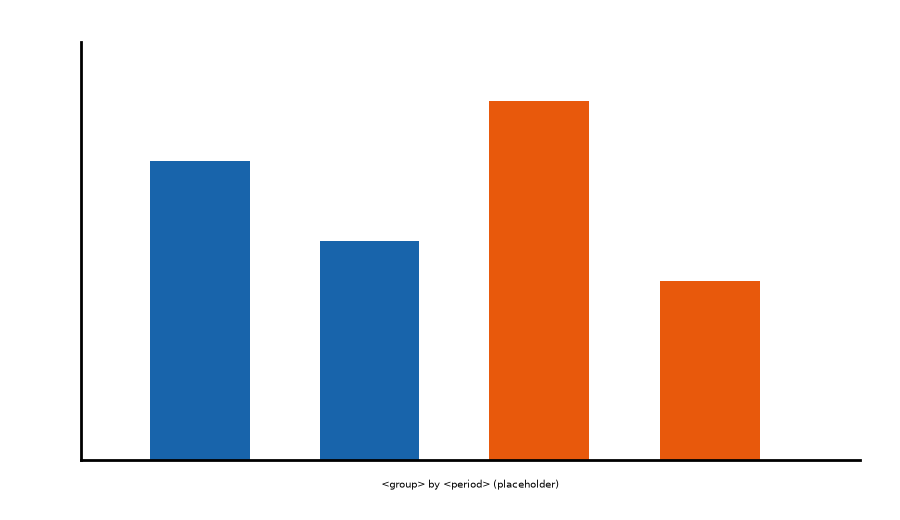
\includegraphics[width=\linewidth]{assets/figure.png}
  \caption{\textbf{<Outcome> by <group>, before and after <the policy>.} Bars show the mean <outcome> per <unit>. Placeholder figure of Tools' Paper-Example; no real data.}
  \label{fig:example}
\end{figure}
}
\clearpage
\section*{What this display says}
\emph{No message written yet: add a ``\#\# Message'' part to method.md (what we want to say with this display), then rerun build\_preview.py.}
\section*{How this display was made}
\subsection*{Data}
<The data source>, years <YYYY to YYYY>.

\subsection*{Sample}
\begin{itemize}\item <who is in it>
\item <how they were chosen>
\end{itemize}
\subsection*{Method}
<The comparison or model, and its estimator.>

\subsection*{Outcomes}
\begin{enumerate}\item \textbf{<outcome>}: <its definition>
\end{enumerate}
\subsection*{Made by}
\begin{itemize}\item \texttt{j02\_evidence\_value/t01\_values-sample/runs/r01\_read\_values/result/values.yaml}, the value Run this display reads (pinned in its run.yaml \texttt{reads:})
\item \texttt{j01\_evidence\_display/t01\_figure1-example/scripts/draw\_figure1.py}
\end{itemize}
\subsection*{Numbers}
Figure 1 prints no number; its bars are placeholder shapes. It reads no value id, so result/values\_used.csv is empty.

\end{document}
